\chapter{Results}
\label{Chap4}
\section{Parameters optimisation}
\label{Rparaopti}
The optimisation of the manufactured samples properties was done with respect to $\rho_{a,rel}$ and $H_v$  by means of $P$ and $v_s$ variation. For this purpose, twelve cubes were fabricated in batch X200-171024. Details about the batch are given in appendix \ref{AppendixA}. The goal of this optimisation was to select a single set of parameters values to use in the rest of the thesis. The parameters values were chosen to cover a wide range of $E_d$. Sets of values of types "7" and "8" are the ones that gave the best results in terms $\rho_{a,rel}$ in a previous work done at UCL. It was decided to produce samples with the corresponding $P$ and $v_s$ in triplicate in order to have a first insight on the process reproducibility.\\

Results for the measurements of $\rho_{a,rel}$ and $H_v$ are displayed in figure \ref{fig:HD-171024}. The 95\% confidence intervals (CI) are also drawn. The methods used to compute them are described in appendix \ref{AppendixC}. All apparent relative density values were obtained trough hydrostatic weighing of the unpolished AB specimens.\\

\begin{figure}[ht]
\centering
\centerline{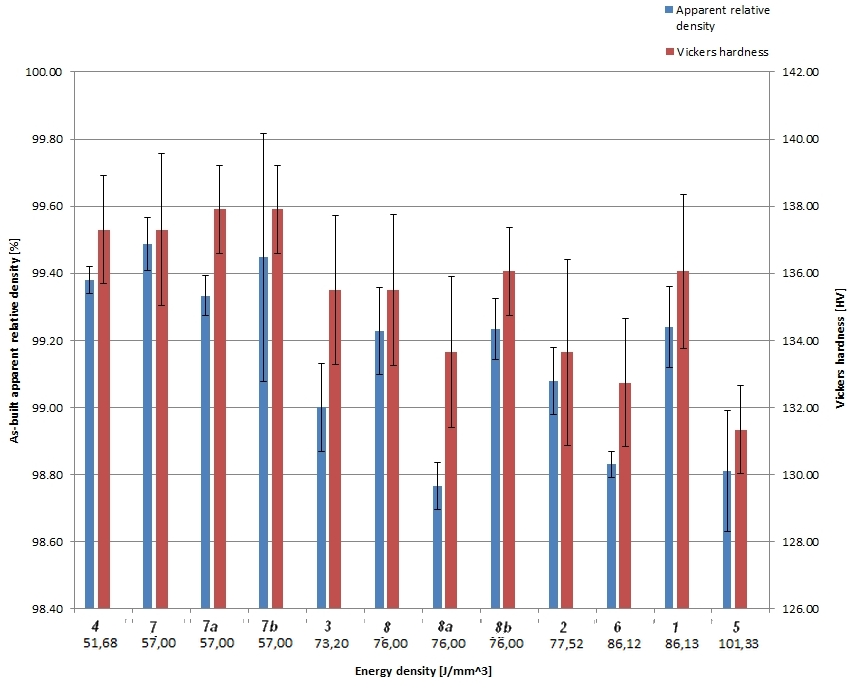
\includegraphics[scale=0.62]{Images/HD-171024}}
\decoRule
\caption[As-built apparent relative density and hardness results for samples of batch X200-171024 as a function of the energy density]{As-built apparent relative density and hardness results for samples of batch X200-171024 as a function of the energy density}
\label{fig:HD-171024}
\end{figure} 

 The graph shows a general progressive decrease of  $\rho_{a,rel}$ and $H_v$ for $E_d>57 [\frac{J}{mm^3}]$. The samples of type "7" have both best $\rho_{a,rel}$ and $H_v$ in average. The standard deviations (SD) of the values are also significantly better than the one of type "8" (see table \ref{tab:78}). One should note that density and hardness values were respectively rounded with four and three significant figures in accordance with the CI sizes. Sample 4 exhibited good properties, comparable to the type "7" specimens. Surprisingly, the worst $\rho_{a,rel}$ measured is that of sample 8a with a value of 98.77[\%].  \\

 \begin{center}
\begin{table}[ht]
\noindent\makebox[\textwidth]{\begin{tabular}{|c|c|c |c |c| c|c|}
    \hline
    Type & $\overline{\rho_{a,rel}}$ [\%] & $SD_{\rho_{a,rel}}$[\%]& $\overline{H_v}$ [HV]& $SD_{H_v}$[HV]\\

\hline
\hline   
    7 & 99.42 & 0.08 & 138 & 0.4 \\
    8 & 99.08 & 0.27 & 135 & 1.3 \\


\hline
\end{tabular}}

\caption[Comparison of standard deviations and average values for apparent relative densities and hardnesses of types 7 and 8 specimens of batch X200-171024]{Comparison of standard deviations and average values for apparent relative densities and hardnesses of types 7 and 8 specimens of batch X200-171024}
\label{tab:78}
\end{table}
 \end{center}

\section{Reproducibility}
\label{RReprod}
\subsection{Relative density and hardness}
\subsubsection{Generalities}

\begin{figure}[ht]
\centering
\centerline{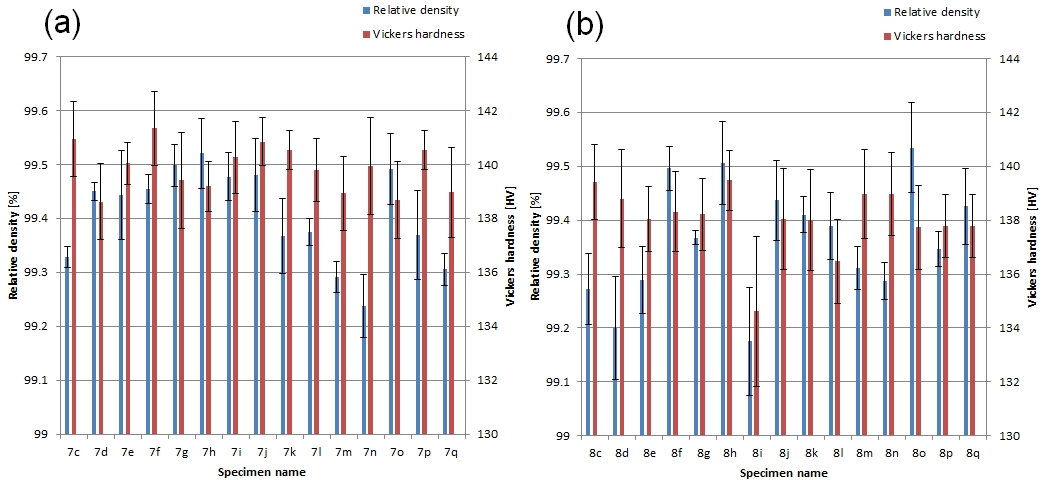
\includegraphics[scale=0.65]{Images/HD-180109-both}}
\decoRule
\caption[As-built apparent relative density and hardness results of batch X200-180109 for (a) type "7" samples (b) type "8" samples.]{As-built apparent relative density and hardness results of batch X200-180109 for (a) type "7" samples (b) type "8" samples.}
\label{fig:HD-171024}
\end{figure} 



\subsubsection{Position influence}


\subsubsection{Sample proximity influence}

\subsubsection{Time influence}

\subsection{Melt pool size and distribution}

\section{Internal properties homogeneity}
As said in section \ref{MMFPP}, all tensile specimens were fabricated vertically. Their height is significantly greater than the other samples'; respectively 6 [cm], and 1 [cm] or less. It was chosen to cut up specimen X200-180417-25 into slices to measure if the density and hardness were homogeneous along the Z direction in the material. The surfaces analysed were named according to their original Z position in the specimen with "B", "C1" , "C2", "C3" and "T" (for bottom, center and top) and to the test done with a letter "D" or "H"  (for density and hardness). The denomination is summarised in figure \ref{fig:saus}.\\

\begin{figure}[ht]
\centering
\centerline{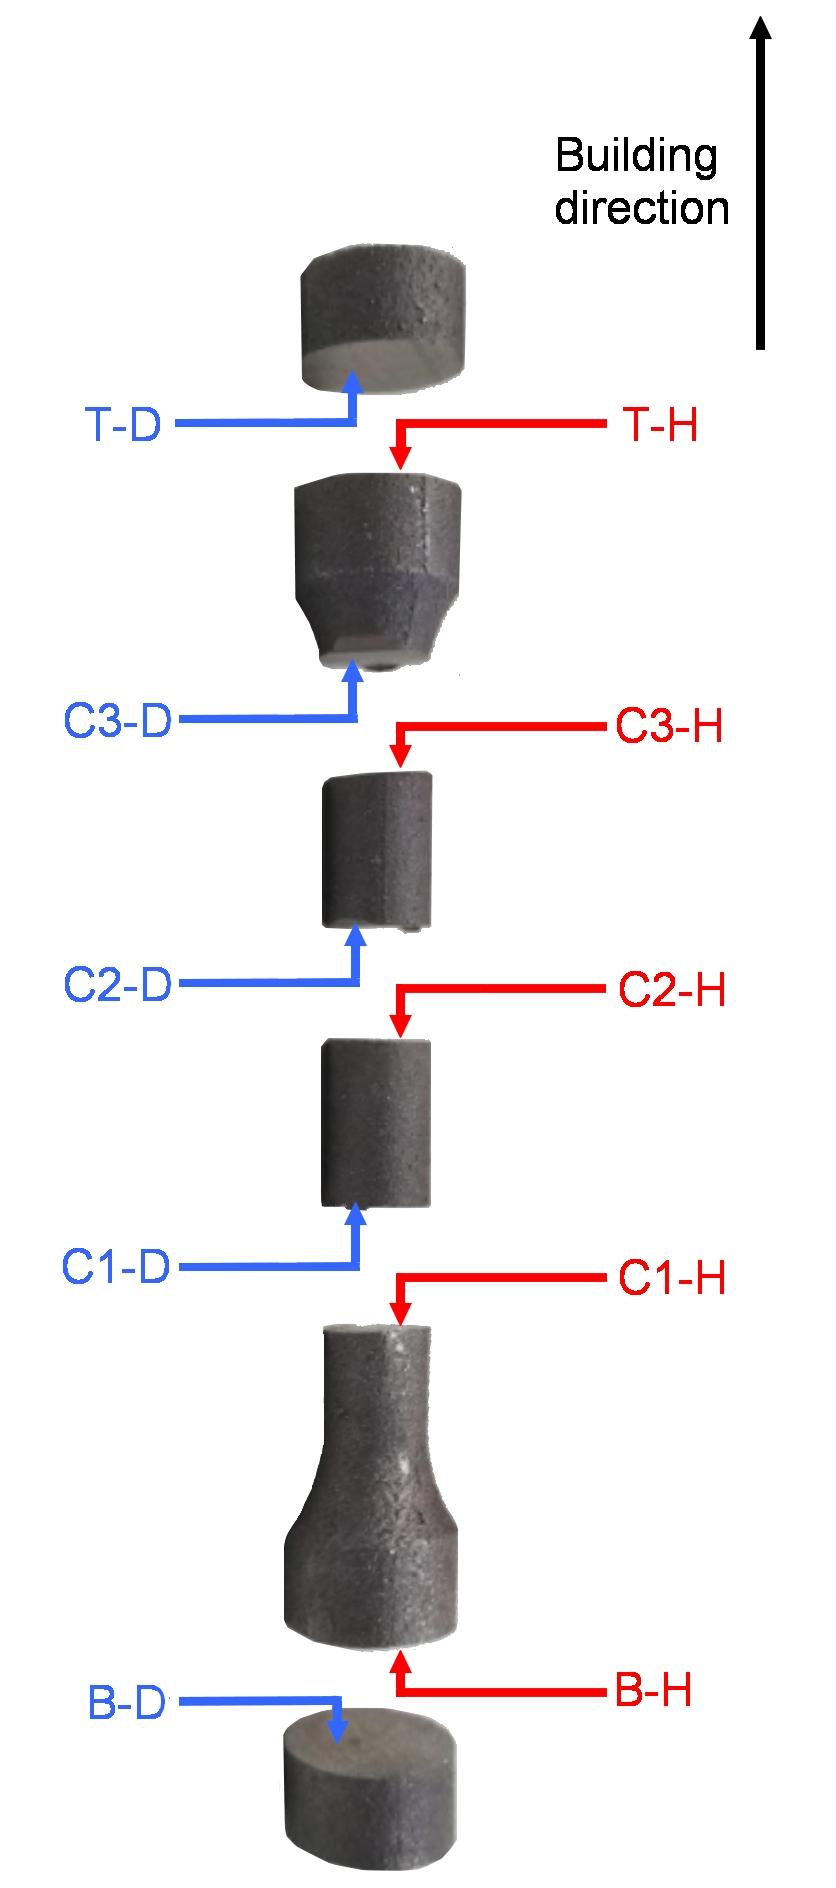
\includegraphics[scale=0.23]{Images/Saus}}
\decoRule
\caption[Specimen X200-180417-25 sub-parts and surfaces denomination]{Specimen X200-180417-25 sub-parts and surfaces denomination.}
\label{fig:saus}
\end{figure}

Results are shown in figure \ref{fig:HD-180417}. With regard to hardness, no general trend could be observed. The measured values are high and closely packed except for the "B" surface, which exhibited a significantly lower hardness. Density values are all equal or above 99.75 [\%]. The values at the center of the sample were slighly lower to the extremities'. A summary of the results is displayed in table \ref{tab:25}.

 \begin{center}
	\begin{table}[ht]
		\begin{tabular}{|c|c |c |c| c|}
			\hline
			Property& Average value & Minimum & Maximum & Standard deviation \\
			\hline 
			\hline   
			Relative density [\%] & 99.80 & 99.75 & 99.87 & 0.05\\
			Hardness [HV] &&&&\\
			\hline
		\end{tabular}
		
		\caption[Relative density and hardness results summary for specimen X200-180417-25 surfaces]{Relative density and hardness results summary for specimen X200-180417-25 surfaces}
		\label{tab:25}
	\end{table}
\end{center}


\begin{figure}[ht]
\centering
\centerline{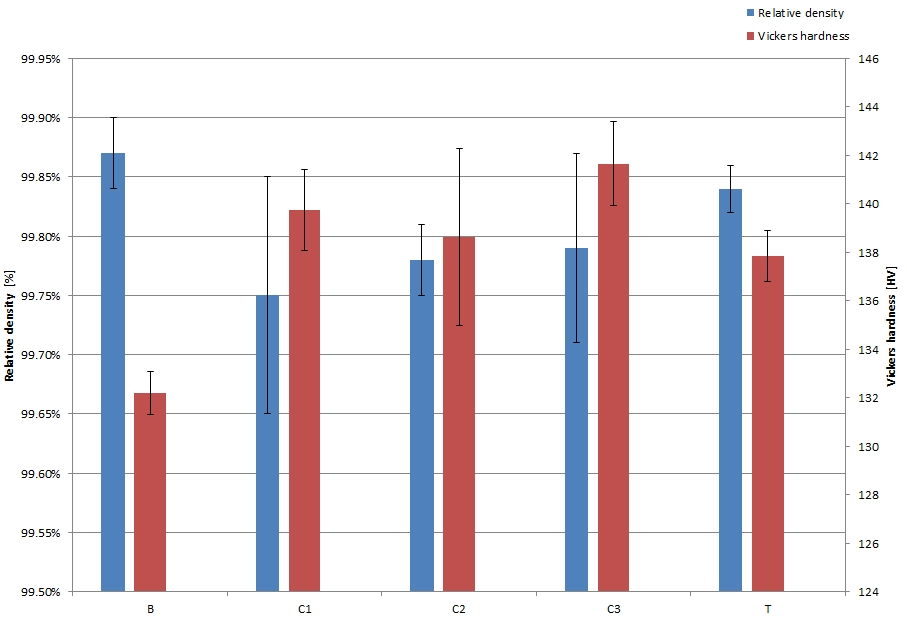
\includegraphics[scale=0.62]{Images/HD-180417}}
\decoRule
\caption[RODIA based relative density and hardness results for specimen X200-180417-25 surfaces]{RODIA based relative density and hardness results for specimen X200-180417-25 surfaces}
\label{fig:HD-180417}
\end{figure} 

\section{Powder ageing}

\subsection{Grain size and distribution}
\subsubsection{Fresh powder}

\subsubsection{Recycled powder}
\subsection{Composition}

\subsubsection{Fresh powder}

\subsubsection{Recycled powder}
 \begin{center}
\begin{table}[ht]
\noindent\makebox[\textwidth]{\begin{tabular}{|c|c |c |c| c|}
    \hline
    Date of sampling& \multicolumn{4}{c}{Composition [\%wt]} \vline\\
    \cline{2-5}
    & Al& Fe&Mg&Si\\
\hline 
\hline   
    23/10/2017  &89.2&0.12&0.49&10.2\\
    09/01/2018 & 89.3 & 0.13 &0.48&10.1\\
    12/01/2018 & 89.4 & 0.13 &0.48&10\\
    21/02/2018&89.1&0.19&0.51&10.3\\
    13/03/2018 &89.1&0.16&0.51&10.1\\    
    \hline
\end{tabular}}

\caption[Composition of recycled AlSi10Mg powder as a function of the date]{Composition of recycled AlSi10Mg powder as a function of the date}
\label{tab:compo}
\end{table}
 \end{center}

\section{Density measures assessments}

\subsection{Measurements comparison}

Several methods were used to measure the densities of the specimens throughout this work: hydrodensimetry (both with and without preliminary polishing) and RODIA. The different techniques were performed on a few specimens in order to draw a comparison of the results and reach a deeper understanding of the methods reliability. The results are gathered on figures ....


\subsection{Relative optical density image analysis}
\label{RRODIA}
One can expect the the density measurement trough RODIA to be a biased method, due to the discretisation in pixels among other things. Results for pictures with different magnifications were compared to quantify these effects. For this purpose, a picture was taken under 5x magnification and two under 10x magnification. The former was delimited to match the visible zones on the latter (see figure \ref{fig:RODIA1}). The same two zones - named A and B - were thus analysed for different levels of resolution.\\

\begin{figure}[ht]
	\centering
	\centerline{\includegraphics[scale=0.075]{Images/RODIA1}}
	\decoRule
	\caption[50x magnification picture of specimen X200-180319-cub1 and delimitation of the zones A and B]{50x magnification picture of specimen X200-180319-cub1 and delimitation of the zones A and B}
	\label{fig:RODIA1}
\end{figure}

\begin{figure}[ht]
	\centering
	\centerline{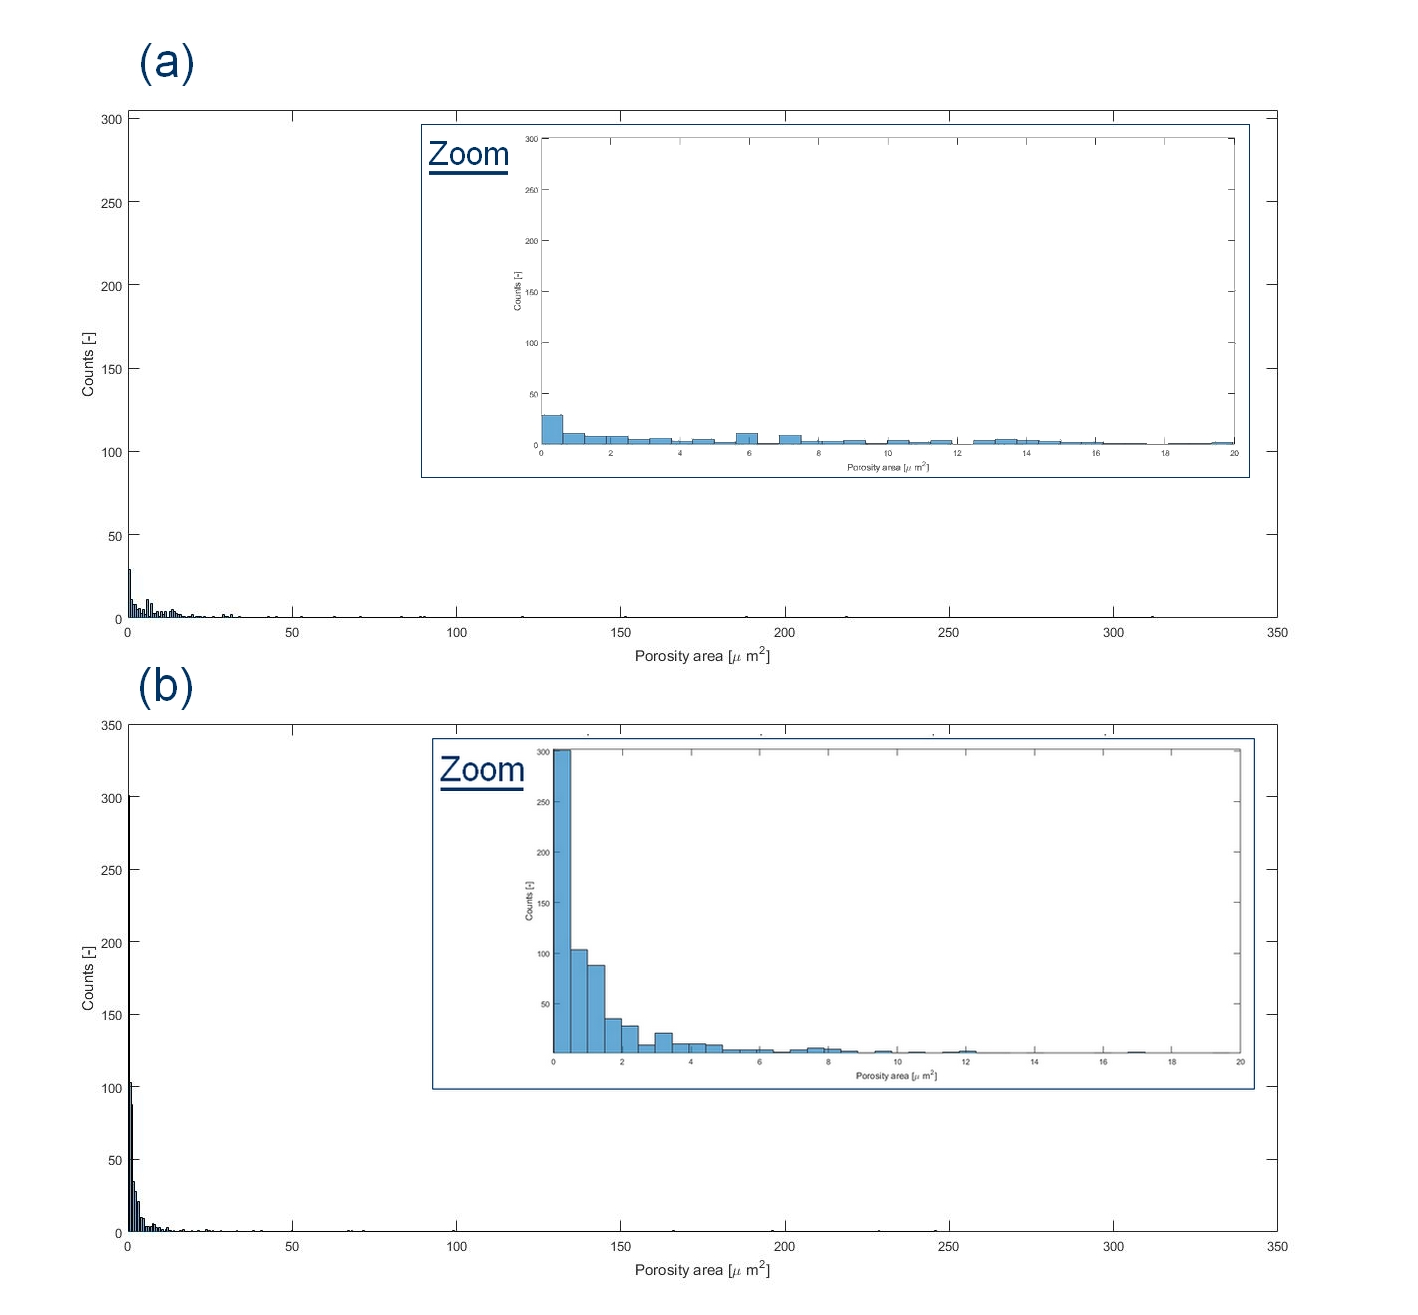
\includegraphics[scale=0.43]{Images/RODIAHist}}
	\decoRule
	\caption[Histograms of porosities areas occurrences from pictures of specimen X200-180319 on zone A under (a) 50x magnification (b) 100x magnification]{Histograms of porosities areas occurrences from pictures of specimen X200-180319 on zone A under (a) 50x magnification (b) 100x magnification. Truncation along the x axis. }
	\label{fig:RODIAH}
\end{figure}


The comparison of figures \ref{fig:RODIA2} (b) and (d) shows that much more small porosities are isolated if the resolution is refined. This is confirmed by the histograms on figure \ref{fig:RODIAH}. The threshold of porosity area for detection in the case of 5x magnification is 7.84 [$\mu m^2$] whereas it is 1.96 [$\mu m^2$] for 10x magnification. This area corresponds to a pixel in each case. It is also worth noting that there is an overall tendency to overestimate the areas at lower resolution, which counterbalances slightly the low number of detected porosities. \\

\begin{figure}[ht]
	\centering
	\centerline{\includegraphics[scale=0.44]{Images/RODIA2}}
	\decoRule
	\caption[Zone A of specimen X200-180319-cub1: (a) Delimitation from original picture under 50x magnification (b) Porosities isolation from 50x magnification picture (c) Original picture under 100x magnification (d) Porosities isolation of 100x magnification picture]{Zone A of specimen X200-180319-cub1: (a) Delimitation from original picture under 50x magnification (b) Porosities isolation from 50x magnification picture (c) Original picture under 100x magnification (d) Porosities isolation of 100x magnification picture}
	\label{fig:RODIA2}
\end{figure}


The RODIA results for zones A and B are outlined in table \ref{tab:RODIASS}. Lower resolution led to the measurement of greater relative densities. The order of magnitude of the difference is of few hundredths of percent.

\begin{center}
	\begin{table}[ht]
		\centerline{\begin{tabular}{|c|c|c|}
				\hline
				Zone & Magnification & Measured relative density [$\%$] \\
				\hline
				A & 50x  & 99.87\\
				A & 100x & 99.84\\
				B & 50x & 99.86\\
				B & 100x & 99.85\\
				\hline
		\end{tabular}}
		\caption[RODIA results for zones A and B of specimen X200-180317 with 50x and 100x magnification]{RODIA results for zones A and B of specimen X200-180317 with 50x and 100x magnification}
		\label{tab:RODIASS}
	\end{table}
\end{center}



\section{Heat treatments}


\subsection{Heating process}

The main objective of most of the research about aluminium alloys AM is to obtain parts with properties at least as good as their conventional cast counterparts. To obtain a larger panel of properties, a vast number of heat treatments have been developed for die cast alloys. The classical treatment of stress-relief for aluminium consists of a heating up to 300$^\circ$ C, with a holding of 2 hours, followed by a slow cooling\ref{label}. This treatment, and variations around him, have been tried on a number of additively manufactured samples, in order to assess their effect on the microstructure and mechanical properties of the parts.\\

A first series of cubic samples was manufactured using the optimised process parameters from Section \ref{Rparaopti}, and a different heat treatment was applied to each one of them. The complete list of cubes treated can be found in Table \ref{RTT}.

\begin{center}
\begin{table}[ht]
\noindent\makebox[\textwidth]{\begin{tabular}{|c|c|c|c|}
	\hline 
	Specimen & Holding time [min] & Aimed holding temp. [$^\circ$C] & Max. temp. [$^\circ$C] \\ 
	\hline 
	X200-180220-TT150-2 & 120 & 150 & - \\ 
	\hline 
	X200-180220-TT200-2 & 120 & 200 & - \\ 
	\hline 
	X200-180220-TT300-2 & 120 & 300 & 256 \\ 
	\hline 
	X200-180220-TT300-2-plaque & 120 & 300 & 281 \\ 
	\hline 
	X200-180220-TT150-2-real & 120 & 150 & 156 \\ 
	\hline 
	X200-180220-TT200-2-real & 120 &200  & 203 \\ 
	\hline 
	X200-180220-TT250-2-real & 120 & 250 & 255 \\ 
	\hline 
	X200-180220-TT300-2-real & 120 & 300 & 302 \\ 
	\hline 
	X200-180220-TT300-1-real & 60 & 300 & 302 \\ 
	\hline 
	X200-180220-TT360-1-real & 60 & 360 & 371 \\ 
	\hline 
	X200-180220-TT300-5m & 5 & 300 & 300 \\ 
	\hline 
\end{tabular}} 
\caption[List of the heat-treated specimens from batch X200-180220]{List of the heat-treated specimens from batch X200-180220}
\label{tab:RTT}
\end{table}
\end{center}

\subsection{Microscopy}

\subsection{Hardness testing}

\subsection{Tensile testing}

 \begin{center}
\begin{table}[ht]
\noindent\makebox[\textwidth]{\begin{tabular}{|c|c|c |c |c| c|c|}
    \hline
    Specimen & Contour &  TT & E [GPa] & $\sigma_y$ [MPa] & $\sigma_u$ [MPa] & $\epsilon_f$[\%] \\

\hline
\hline   
    X200-180417-1 & Yes & None & (74.6) & 260.8 & 366.4 & 2.2  \\
    X200-180417-2 & Yes & None & 68.2 & 290.2 & 388.3 & 2.4\\
    X200-180417-3 & Yes & None & 64.7 & 275.9 & - & - \\    
    
    X200-180417-16 & Yes & None & 64.7  & 255.8  & 368.0 &2.3 \\ 
    
    X200-180417-17 & Yes & None & 66.1   & 250.1  &  406.4&3.0  \\ 
    
    X200-180417-A & No & None & 62.0 &257.1  & 379.2 & 2.8 \\
    
    X200-180417-13 & Yes & 150$^\circ$C (2h) & 70.9  & 299.5 & 436.2 & 5.1  \\    
    X200-180417-14 & Yes & 150$^\circ$C (2h) & 67.9 & 304.5  &442.7  & 5.2  \\    
    %X200-180417-15 & Yes & 150$^\circ$C (2h) &  &  &  &  \\    
    X200-180417-B & Yes & 150$^\circ$C (2h) & 66.5 & 288.0  & 446.2 &6.3  \\    
    X200-180417-10 & Yes & 200$^\circ$C (2h) &72.5  &253.4  & 393.4  &4.9  \\    
    X200-180417-11 & Yes & 200$^\circ$C (2h) &71.7  &242.5  &370.6  &4.3  \\    
    %X200-180417-12 & Yes & 200$^\circ$C (2h) &  &  &  &  \\    
    X200-180417-S-8 & Yes& 250$^\circ$C (2h) & 69.6 & 238.9 & 347.4 & 8.6 \\
    X200-180417-9 & Yes& 250$^\circ$C (2h) & 71.0 & 227.7 &$\simeq 328.7$ & - \\
    X200-180417-4 & Yes& 300$^\circ$C (2h) & (81.6) & 164.4 & 249.6 & 14.1 \\ 
    X200-180417-5 & Yes& 300$^\circ$C (2h) & 68.3 &172.4 & 256.24 & 13.1 \\
    X200-180417-6 & Yes& 300$^\circ$C (2h) & 69.5 &168.5 & $\simeq 242.5$ & - \\

\hline
\end{tabular}}

\caption[Tensile mechanical properties of the specimens from batch X200-180417]{Tensile mechanical properties of the specimens from batch X200-180417}
\label{tab:pol}
\end{table}
 \end{center}
 
\subsection{Internal stress testing}





%\begin{table}
%\caption{The effects of treatments X and Y on the four groups studied.}
%\label{tab:treatments}
%\centering
%\begin{tabular}{l l l}
%\toprule
%\tabhead{Groups} & \tabhead{Treatment X} & \tabhead{Treatment Y} \\
%\midrule
%1 & 0.2 & 0.8\\
%2 & 0.17 & 0.7\\
%3 & 0.24 & 0.75\\
%4 & 0.68 & 0.3\\
%\bottomrule\\
%\end{tabular}
%\end{table}